\section{De applicatielaag: Sequentie- en Collaboratie diagram}

De sequentie- en collaboratiediagrammen zijn de volgende dynamische diagrammen in UML, ze worden ook wel \textbf{interactiediagrammen} genoemd. 

In deze diagrammen vind je de interacties die tussen de verschillende objecten optreden.

Zowel het sequentie- als het collaboratiediagram neemt de use-case als uitgangspunt en zullen informatie vastleggen over het interne gedrag van het systeem. Ze geven inzicht in de interactie tussen de objecten die nodig is voor het verwezenlijken van het systeem. Ze stellen de dynamische samenwerking tussen objecten voor. Het scenario zoals beschreven in de use-case beschrijving wordt vertaald naar de reeks berichten die tussen objecten verzonden worden.

In het sequentiediagram beschrijft men de tijdsdynamica van de interactie, 

terwijl je in het collaboratiediagram aangeeft op welke manier de verschillende klassen met elkaar samenwerken. 

Je vindt exact dezelfde informatie terug in de beide diagrammen, maar de manier van benadrukken is anders.

\subsection{Concepten van het sequentiediagram}
Het sequentiediagram toont de dynamische samenwerking tussen verschillende objecten.

Het belang van dit diagram is het geven van het overzicht van de berichten die tussen verschillende objecten worden verzonden in het kader van een use-case. 

Het diagram bestaat uit een aantal objecten met verticale lijnen.

In deze \textbf{verticale} lijnen wordt het tijdsverloop weergegeven 

en in de \textbf{horizontale} lijnen wordt de uitwisseling van berichten getoond.

Volgende concepten zijn van belang bij het opmaken van een sequentiediagram :

\subsubsection{interactie: EXAMENVRAAG}

\textcolor{red}{Een interactie is een reeks van gebeurtenissen die plaats vinden tijdens één specifieke sessie met het systeem.}

In de use-case werden de verschillende interactiestappen uitgewerkt. Uitgaande van deze interactie tussen de actor en het systeem wordt nu deze interactie beschreven met behulp van events tussen objecten. \textcolor{red}{Dat systeem dat in de use-cases beschouwd werd als een black box wordt nu een white box en met behulp van de objecten uitgediept.}

\subsubsection{ gebeurtenis (event)}
Een event is een gebeurtenis die geen tijd kost, ze kan niet opgedeeld worden. Dit heeft tot gevolg dat een event of gebeurd is, of nog moet gebeuren. Voorbeeld, een operatie aanroepen of een boodschap sturen.

%afbeelding nog plaatsen

\begin{center}
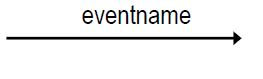
\includegraphics[width=4in]{img/event1}
\end{center}

Een interactie is een opeenvolging van events.
In het sequentiediagram wordt een event weergegeven als een pijl met een eventnaam bij. In het collaboratiediagram vind je een event voorgesteld als een eventnaam met een klein pijltje erboven of ernaast.

In een collaboratiediagram wordt een gebeurtenis als volgt voorgesteld:

%afbeelding nog plaatsen

\begin{center}
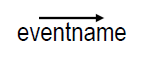
\includegraphics[width=4in]{img/event2}%
\end{center}

\subsubsection{tijdsconstraint}

In een sequentiediagram kan het nodig zijn om een beperking aan te geven op het tijdsverloop van twee events.
Dergelijk tijdsconstraint geef je aan in de kantlijn van het sequentiediagram, in het collaboratie diagram kan je geen tijdsconstraint aantreffen, aangezien hier niet de nadruk op het tijdsaspect maar wel op de samenwerking valt..

\subsubsection{asynchroon event}

Een asynchroon event is een event dat door het ontvangend object niet verwerkt wordt op het moment van verzending.
In het sequentiediagram wordt een asynchroon event weergegeven door de pijl die de event weergeeft schuin naar beneden te laten lopen (i.p.v. horizontaal).

%afbeelding nog plaatsen

\begin{center}
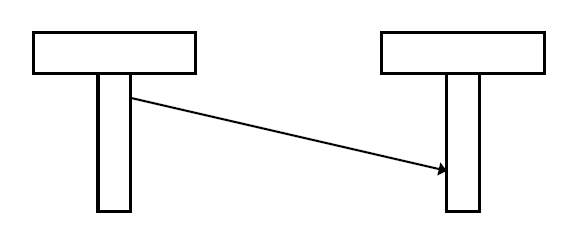
\includegraphics[width=4in]{img/async1}%
\end{center}

In het collaboratiediagram wordt een asynchroon event aangeduid door een pijl met een halve pijlpunt.

%afbeelding nog plaatsen

\begin{center}
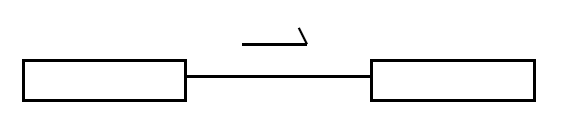
\includegraphics[width=4in]{img/async2}%
\end{center}

\subsubsection{conditionele event}

Met een conditionele event bedoelt men een gebeurtenis die slechts onder bepaalde condities mag voorkomen. De gebeurtenis zal dus enkel doorgaan als de conditie voldaan is.

Voorbeeld. In een bank mag ik enkel geld van mijn zichtrekening halen als het saldo na afhalen niet onder een bepaalde limiet gaat.

In het sequentiediagram geef je een conditionele event weer als een logische expressie tussen rechte haken.

%afbeelding nog plaatsen

\begin{center}
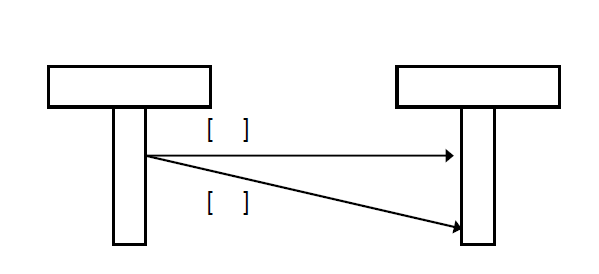
\includegraphics[width=4in]{img/cond1}%
\end{center}

In het collaboratiediagram wordt de conditionele event ook tussen vierkante haakjes geplaatst.

%afbeelding nog plaatsen

\begin{center}
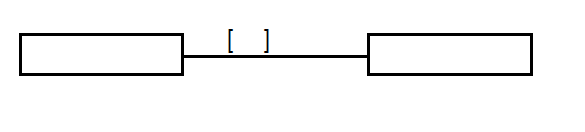
\includegraphics[width=4in]{img/cond2}%
\end{center}

\subsubsection{Iteratie van events}

Vaak moet een bericht meermaals verstuurd worden, bvb. met een andere parameter. Dergelijke iteratie geef je als volgt aan : een sterretje geeft de iteratie weer en tussen twee rechte haken staan de iteratiewaarden.

In het sequentiediagram:

%afbeelding nog plaatsen

\begin{center}
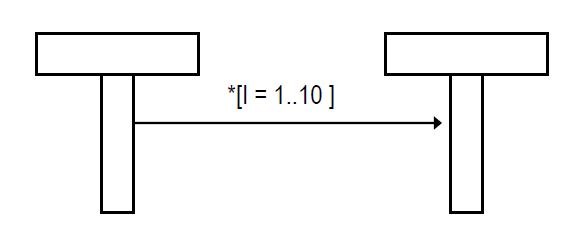
\includegraphics[width=4in]{img/iter1}%
\end{center}

In het collaboratiediagram:

%afbeelding nog plaatsen

\begin{center}
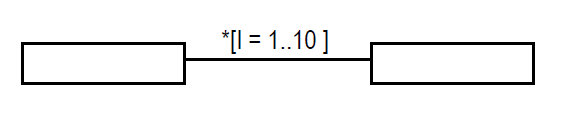
\includegraphics[width=4in]{img/iter2}%
\end{center}

\subsubsection{activering van een object}

Een actief object is een object dat uit zichzelf acties kan uitvoeren of berichten kan versturen.
De tijdsperiode waarin een object een actie uitvoert wordt weergegeven door een witte balk in het sequentiediagram. In het coliaboratiediagram kan je de tijd niet aangeven, maar je kan wel aangeven dat een object geactiveerd wordt, een actief object wordt weergegeven als een object waarvan de rand vet is.

In het sequentiediagram:

%afbeelding nog plaatsen

\begin{center}
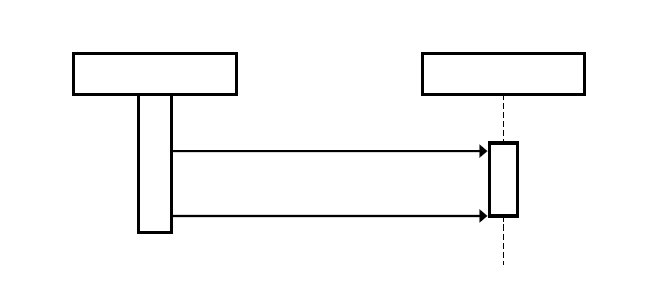
\includegraphics[width=4in]{img/activ1}%
\end{center}

In het coliaboratiediagram:

%afbeelding nog plaatsen

\begin{center}
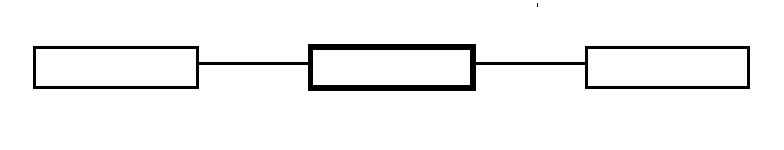
\includegraphics[width=4in]{img/activ2}%
\end{center}

\subsubsection{creatie of verwijdering van objecten}

Ook de creatie of verwijdering van objecten kan weergegeven worden.
De creatie van een object geef je in een sequentiediagram aan door de pijl die de event aangeeft niet naar de witte balk van het object te laten gaan maar naar de rechthoek daarboven. De verwijdering van een object wordt aangeduid door een groot, dik kruis te tekenen aan het einde van de balk.

%afbeelding nog plaatsen


\begin{center}
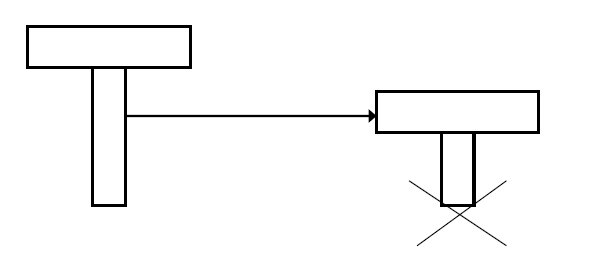
\includegraphics[width=4in]{img/destr1}%
\end{center}


In het collaboratiediagram geef je m.b.v. \big\{new\big\} aan dat het object gecreëerd wordt, \big\{destroyed\big\} geeft aan dat het verwijderd wordt en {\big\{transient\big\} is een afkorting voor \big\{new destroyed\big\}, wat betekent: zowel gecreëerd als opnieuw verwijderd tijdens dezelfde interactie.

%afbeelding nog plaatsen

\begin{center}
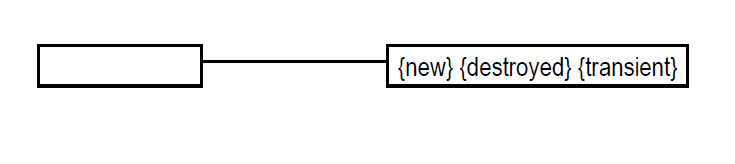
\includegraphics[width=4in]{img/destr2}%
\end{center}

\subsubsection{recursie of zelfaanroep}

Indien een object een operatie op zichzelf aanroept, spreekt men over recursie.

%afbeelding nog plaatsen

\begin{center}
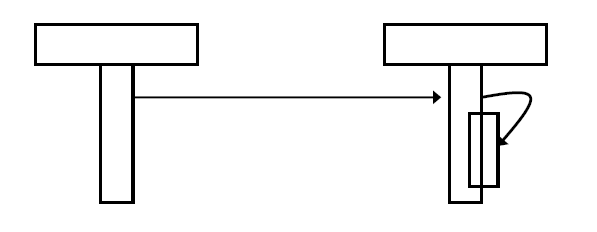
\includegraphics[width=4in]{img/rec1}%
\end{center}

Dergelijke recursie wordt in beide diagrammen aangeduid door een kromme lijn, bij het sequentiediagram heeft de lijn een pijlpunt en gaat de pijl van de witte balk naar een nieuwe witte balk die gedeeltelijk over de eerste ligt.

%afbeelding nog plaatsen

\begin{center}
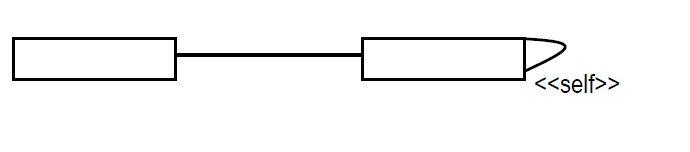
\includegraphics[width=4in]{img/rec2}%
\end{center}

In het collaboratiediagram staat naast de kromme lijn het stereotype <<self>>.

\subsubsection{resultaat van een operatieaanroep}

Indien het zinvol is om het resultaat van een operatieaanroep op te nemen, doet men dit als volgt : in het sequentiediagram geef je het resultaat aan m.b.v. een onderbroken pijl. Bij deze pijl staat een symbolische naam.

%afbeelding nog plaatsen

\begin{center}
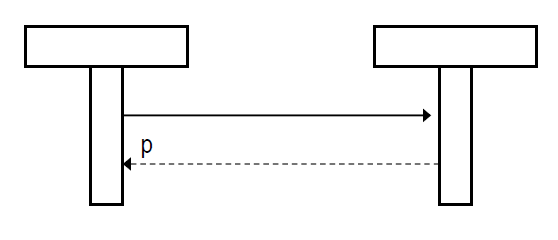
\includegraphics[width=4in]{img/result1}%
\end{center}

In het collaboratiediagram wordt de waarde als het ware "toegekend"  aan een variabele die in het vervolg van de interactie gebruikt kan worden.

%afbeelding nog plaatsen

\begin{center}
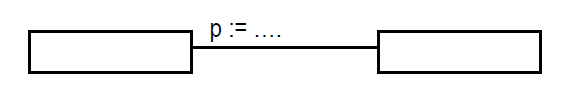
\includegraphics[width=4in]{img/result2}%
\end{center}

Het sequentiediagram toont de interactie met de nadruk op het \textbf{tijdsaspect}. 

Op het sequentiediagram worden de events tussen de objecten aangegeven. 

Veel van deze events zullen later gemodelleerd worden als operaties bij de klasse van het object dat ze ontvangt, let dus nu al op de naamgeving van de events.

Om het sequentiediagram te tekenen plaats je bovenaan de objecten die aangeroepen zullen worden bij de uitwerking van de use-case. De volgorde is willekeurig maar wordt best zo gekozen dat het schema zo duidelijk mogelijk is.

Bij elk object teken je de levenslijn van het object waarbij de berichten verstuurd worden van object naar object.

\subsection{Sequentiediagram : hoe opstellen ?}

Om het sequentiediagram op te stellen, volgt men de volgende werkwijze :

\begin{enumerate}
\item Kies de use-case die uitgewerkt moet worden en uit de paden het pad dat uitgewerkt moet worden


Voor de uit te werken use-case wordt het te volgen pad bepaald. Dit kan je terugvinden in de tekstuele beschrijving van de use-case.
\item Bepaal naar welk object de actor zijn boodschap stuurt


Allereerst wordt er bepaald welk object het verzoek van de gebruiker aanneemt. Het is aan te raden hiervoor een user interface object te introduceren zodat het onderscheid behouden blijft tussen het bedrijfsmodel en de manier waarop de eindgebruiker het systeem te zien krijgt.
\item Bepaal de beantwoording door het object


Er wordt nagegaan of het object de gevraagde service kan leveren. Indien dit het geval is, wordt deze via een event van het object naar de gebruiker gezonden. Indien het object informatie nodig heeft van andere objecten, dan stuurt het een boodschap naar een ander object
\item Herhaal stap 3 voor alle objecten die een event ontvangen


Deze derde stap wordt herhaald voor alle objecten die in de interactie opgeroepen worden, waarbij elk object, dat nodig blijkt, toegevoegd wordt.
\item Bepaal eventuele condities, asynchrone communicatie, tijdsbeperkingen enz.


Indien condities, asynchrone events enz. nodig blijken te zijn, worden deze toegevoegd.
\end{enumerate}


\subsection{Het collaboratiediagram}

Het collaboratiediagram toont, net als het sequentiediagram, \textcolor{red}{een dynamische samenwerking tussen objecten.}

Dit diagram toont de

\begin{itemize}
    \item interactie (uitwisseling van berichten)
    \item en de context (objecten en relaties)
\end{itemize}

Daar waar het sequentiediagram de \textbf{nadruk} legt op het \textcolor{red}{\textbf{tijdsverloop}}, 

wordt in het collaboratiediagram het tijdsaspect terzijde gelaten en de nadruk gelegd op de context, de samenwerking.

Ook bij het collaboratiediagram wordt de \textbf{use-case als uitgangspunt} genomen waarbij men het collaboratiediagram gebruikt om de onderlinge samenwerking van de objecten uit te tekenen om tot een bepaald doel te komen nl. het uitvoeren van de functionaliteit beschreven in de use-case.

\subsection{collaboratie- of sequentiediagram ?}

Om uit te maken hoeveel en welke diagrammen je best tekent, houd je rekening met de volgende richtlijnen :

\begin{itemize}
    \item voor elke use-case maak je minstens één sequentie- of collaboratiediagram.
    \item voor elke keuze in een use-case die een \textbf{relevant verschil} maakt voor het\textbf{ vervolg van de use-case} maak je een apart sequentie- of collaboratiediagram
\end{itemize}

\subsection{het gebruik van CRC-kaarten}

Om het maken van sequentie- en collaboratiediagrammen te vergemakkelijken kan men de interactie als een soort rollenspel naspelen in een groep ontwikkelaars. Hierbij is een CRC-kaart een kaartje waarop voor één klasse alle verantwoordelijkheden en samenwerkingsverbanden staan.

Deze kaarten worden gebruikt tijdens een workshop: elke persoon ontvangt een kaart en vereenzelvigt zich met de klasse die op de kaart vermeld wordt. Vervolgens zal de spelleider de externe actor spelen en begint : het eerste object voor de beantwoording van de vraag wordt gezocht. Als deze persoon zelf het antwoord kan geven zal dit gebeuren, zo niet wordt de vraag verder gesteld aan een ander object enz.

Indien men tijdens dergelijk workshop ontdekt dat de verantwoordelijkheid voor het beantwoorden van de vraag bij geen van de aanwezige klassen te plaatsen is, betekent dit dat een extra klasse toegevoegd moet worden aan het klassendiagram. Op deze manier zal men ook komen tot het toevoegen van attributen of operaties.

\subsection{Terugkoppeling naar klassendiagram}

Voor elk sequentie- en collaboratiediagram moet terug gekoppeld worden naar het klassendiagram:
\begin{itemize}
    \item De nieuwe toegevoegde klassen moeten in het klassendiagram toegevoegd worden en de juiste relaties moeten gelegd worden.
    \item Elk event dat voorkomt in het sequentie- of collaboratiediagram moet als operatie opgenomen worden in de klassen van het object waarbinnen het event binnen komt
\end{itemize}

